\hypertarget{extended-kalman-filter}{%
\section{\texorpdfstring{\texttt{Extended\ Kalman\ Filter}}{Extended Kalman Filter}}\label{extended-kalman-filter}}

Recall that when we started the section on linear dynamical systems the
first example was the differential drive dynamics. These equations are
not linear due to the cos and sin terms. What does one do in the case
where the process or the observation is a nonlinear function? For a
nonlinear process, let \(x_k \in R^n\), \(u_k \in R^p\),
\(v_k  \in R^n\), \(w_k  \in R^m\),

\[x_k = f(u_k,x_{k-1}) + v_k,\]

\[z_k = h(x_{k-1})+w_k\]

where \(v_k\) has variance \(V_k\) and \(w_k\) has variance \(W_k\), and
let

\[\begin{aligned}
F_k = \partial f / \partial x = \displaystyle
  \begin{bmatrix} \frac{\partial f_1}{\partial x_1} & \frac{\partial f_1}{\partial x_2}  & \dots &
\frac{\partial f_1}{\partial x_n}  \\[8pt]
\frac{\partial f_2}{\partial x_1} & \frac{\partial f_2}{\partial x_2}  & \dots &
\frac{\partial f_2}{\partial x_n}  \\[8pt] \vdots & \vdots & \vdots \\[8pt]
\frac{\partial f_n}{\partial x_1} & \frac{\partial f_n}{\partial x_2}  & \dots &
\frac{\partial f_n}{\partial x_n}  \end{bmatrix},
\displaystyle H_k = \begin{bmatrix} \frac{\partial h_1}{\partial x_1} & \frac{\partial h_1}{\partial x_2}  & \dots &
\frac{\partial h_1}{\partial x_n}  \\[8pt]
\frac{\partial h_2}{\partial x_1} & \frac{\partial h_2}{\partial x_2}  & \dots &
\frac{\partial h_2}{\partial x_n}  \\[8pt] \vdots & \vdots & \vdots \\[8pt]
\frac{\partial h_m}{\partial x_1} & \frac{\partial h_m}{\partial x_2}  & \dots &
\frac{\partial h_m}{\partial x_n}  \end{bmatrix}
\end{aligned}\]

This is a \texttt{Taylor\ expansion} approach to dealing with nonlinear
mappings. For more information about \texttt{Jacobians},
\url{https://en.wikipedia.org/wiki/Jacobian_matrix_and_determinant}.

\begin{enumerate}
\item
  Predicted state:

  \[\hat{x}_{k|k-1} = f(\hat{x}_{k-1|k-1}, u_{k})\]
\item
  Predicted estimate covariance:

  \[P_{k|k-1} = F_{k} P_{k-1|k-1} F_{k}^{T} + V_{k}\]
\item
  Optimal Kalman gain:

  \[K_k = P_{k|k-1}H_k^\text{T}\left(H_k
  P_{k|k-1} H_k^\text{T} + W_k\right)^{-1}\]
\item
  Updated state estimate:

  \[\hat{x}_{k|k} =\hat{x}_{k|k-1} + K_k \left(z_k - h(\hat{x}_{k|k-1})\right)\]
\item
  Updated estimate covariance:

  \[P_{k|k} =
    (I - K_k H_k) P_{k|k-1}\]
\end{enumerate}

Summed up into a procedure, we have:

\begin{quote}
\textbf{Input} \(x_0\), \(P_0\)\\
\textbf{Output} Estimates of \(x_k\), \(P_k\)\\
\(k=0\)\\
\textbf{while} (not terminated) \textbf{do}\\
\hspace*{0.333em}\hspace*{0.333em}\hspace*{0.333em}\(k=k+1\)\\
\hspace*{0.333em}\hspace*{0.333em}\hspace*{0.333em}\(x_k = f(\hat{x}_{k-1|k-1}, u_{k})\)\\
\hspace*{0.333em}\hspace*{0.333em}\hspace*{0.333em}\(F_k =  \mbox{Jacobian}(f)|_{x_k}\)\\
\hspace*{0.333em}\hspace*{0.333em}\hspace*{0.333em}\(P_{k} = F_{k} P_{k-1} F_{k}^{T} + V_{k}\)\\
\hspace*{0.333em}\hspace*{0.333em}\hspace*{0.333em}\(H_k = \mbox{Jacobian}(h)|_{x_k}\)\\
\hspace*{0.333em}\hspace*{0.333em}\hspace*{0.333em}\(y_k = z_k - H_k x_{k}\)\\
\hspace*{0.333em}\hspace*{0.333em}\hspace*{0.333em}\(S_k = H_k P_{k} H_k^\text{T} + W_k\)\\
\hspace*{0.333em}\hspace*{0.333em}\hspace*{0.333em}\(K_k = P_{k}H_k^\text{T}S_k^{-1}\)\\
\hspace*{0.333em}\hspace*{0.333em}\hspace*{0.333em}\(x_k =   x_{k} + K_k y_k\)\\
\hspace*{0.333em}\hspace*{0.333em}\hspace*{0.333em}\(P_{k} = (I - K_k H_k) P_{k}\)\\
\textbf{end while}
\end{quote}

\hypertarget{short-example}{%
\subsection{Short Example}\label{short-example}}

What is the Extended Kalman Filter formulation of the motion model:

\[\begin{aligned}
\begin{array}{l}\dot{x} = y \\\dot{y} = -\cos(x) + 0.4\sin(t)\end{array},
\end{aligned}\]

and observation

\[\begin{aligned}
h(x,y) = \begin{bmatrix}x \\ y\end{bmatrix}
\end{aligned}\]

with step size \(\Delta t = 0.1,\) and noise

\[\begin{aligned}
V = \begin{bmatrix} 0.1&0.01\\0.01& 0.1\end{bmatrix}, \quad , W = \begin{bmatrix} 0.05&0\\0& 0.05\end{bmatrix}.
\end{aligned}\]

Assume that the initial values, \(t_0 = 0\),

\[\begin{aligned}
x_0 = \begin{pmatrix} 1 \\ 1 \end{pmatrix}
\end{aligned}\]

and we have a reasonably accurate start

\[\begin{aligned}
P_0 = \begin{pmatrix} 0.5 & 0 \\ 0 & 0.5   \end{pmatrix}
\end{aligned}\]

Using a basic Euler formulation we replace the derivative:

\[\begin{aligned}
\begin{array}{l}\displaystyle\frac{x_{k+1} - x_k}{0.1} = y_k \\[3mm]
\displaystyle\frac{y_{k+1} - y_k}{0.1} = -\cos(x_k) + 0.4\sin(t_k)\end{array}
\end{aligned}\]

This gives the discrete form:

\[\begin{aligned}
\begin{array}{l}x_{k+1} = x_k + 0.1 y_k \\y_{k+1} = y_k -0.1\cos(x_k) + 0.04\sin(t_k)\end{array}
\end{aligned}\]

and so

\[\begin{aligned}
F = \begin{bmatrix} 1 & 0.1 \\ 0.1\sin(x_k) & 1 \end{bmatrix},  \quad
H = \begin{bmatrix} 1 & 0 \\ 0 & 1 \end{bmatrix}
\end{aligned}\]

\textbf{EKF:}

\begin{enumerate}
\item
  Predicted state:

  \[\begin{aligned}
  \hat{x}_{1|0} = f(\hat{x}_{0|0}, u_{1})  =\begin{pmatrix} 1+0.1(1) \\ 1 - 0.1\cos(1) + 0.04\sin(0) \end{pmatrix} =   \begin{pmatrix} 1.1 \\ 0.45969769\end{pmatrix}
  \end{aligned}\]
\item
  Predicted estimate covariance:

  \[P_{1|0} = F_{1} P_{0|0} F_{1}^{T} + V_{1}\]

  \[\begin{aligned}
  =  \begin{bmatrix} 1 & 0.1 \\ 0.1\sin(1) & 1 \end{bmatrix}   \begin{bmatrix} 0.05 & 0 \\ 0 & 0.05   \end{bmatrix} \begin{bmatrix} 1 & 0.1\sin(1) \\ 0.1 & 1 \end{bmatrix} +
  \end{aligned}\]

  \[\begin{aligned}
  \begin{bmatrix} 0.1&0.01\\0.01& 0.1\end{bmatrix}
  =  \begin{bmatrix} 0.605   &    0.10207355 \\
   0.10207355  &  0.60354037 \end{bmatrix}
  \end{aligned}\]
\item
  Optimal Kalman gain:

  \[K_1 = P_{1|0}H_1^\text{T}\left(H_1
  P_{1|0} H_1^\text{T} + W_1\right)^{-1}\]

  \[\begin{aligned}
  =  \begin{bmatrix} 0.605   &    0.10207355 \\
   0.10207355  &  0.60354037 \end{bmatrix}
  \end{aligned}\]

  \[\begin{aligned}
  \times \left(  \begin{bmatrix} 0.605   &    0.10207355 \\
   0.10207355  &  0.60354037 \end{bmatrix}  + \begin{bmatrix} 0.05&0\\0& 0.05\end{bmatrix}\right)^{-1}
  \end{aligned}\]

  \[\begin{aligned}
  = \begin{bmatrix} 0.92175979 & 0.01221999 \\
          0.01221999 &  0.92158505 \end{bmatrix}
  \end{aligned}\]
\item
  Updated state estimate:

  \[\hat{x}_{1|1} =\hat{x}_{1|0} + K_1 \left(z_1 - h(\hat{x}_{1|0})\right)\]

  \[\begin{aligned}
  =\begin{pmatrix} 1.1 \\ 0.45969769\end{pmatrix} + \begin{bmatrix} 0.92175979 & 0.01221999 \\
          0.01221999 &  0.92158505 \end{bmatrix}
  \end{aligned}\]

  \[\begin{aligned}
  \times \left(\begin{pmatrix}1.15 \\ 0.5\end{pmatrix} -  \begin{pmatrix} 1.1 \\ 0.45969769 \end{pmatrix} \right)
    =  \begin{pmatrix} 1.14658048 \\ 0.4974507 \end{pmatrix}
  \end{aligned}\]
\item
  Updated estimate covariance:

  \[P_{1|1} =
    (I - K_1 H_1) P_{1|0}\]

  \[\begin{aligned}
  = \left( \begin{pmatrix}1&0\\0&1\end{pmatrix} -  \begin{bmatrix} 0.92175979 & 0.01221999 \\
          0.01221999 &  0.92158505 \end{bmatrix}\right)
  \end{aligned}\]

  \[\begin{aligned}
  \times \begin{bmatrix} 0.605   &    0.10207355 \\
   0.10207355  &  0.60354037 \end{bmatrix} =
  \begin{bmatrix} 0.04608799&  0.000611 \\
          0.000611  &  0.04607925 \end{bmatrix}
  \end{aligned}\]
\end{enumerate}

\hypertarget{differential-drive-example}{%
\subsection{Differential Drive
Example}\label{differential-drive-example}}

In Terms Chapter, we derived the equations for the motion of the
differential drive robot. In that chapter we also simulated the motion
of the robot based on wheel velocity data. Small amounts of noise in the
wheel velocity data could cause significant errors in position
estimation. Using the Extended Kalman Filter, we can improve the
location estimate as well as gain estimates for the uncertainty of the
location. \texttt{Fig:DDagain} recalls the variables and equations that
were derived.

\begin{quote}
The variables used in the DD model.
\end{quote}

\[\begin{aligned}
\begin{array}{l}
 \dot{x} = \frac{r}{2} (\dot{\phi_1}+\dot{\phi_2})\cos(\theta) \\[5mm]
\dot{y} = \frac{r}{2} (\dot{\phi_1}+\dot{\phi_2})\sin(\theta) \\[5mm]
\dot{\theta} = \frac{r}{2L} (\dot{\phi_1}-\dot{\phi_2})
\end{array}
\end{aligned}\]

As with the linear continuous models, both the Kalman and Extended
Kalman filters act on discrete dynamics. So as before, we need to
discretize the equations.

\[\begin{aligned}
\begin{array}{l}
\displaystyle \frac{x(t+\Delta t) - x(t)}{\Delta t}\approx \dot{x} = \frac{r}{2} (\dot{\phi_1}+\dot{\phi_2})\cos(\theta) \\[5mm]
\displaystyle \frac{y(t+\Delta t) - y(t)}{\Delta t}\approx \dot{y} = \frac{r}{2} (\dot{\phi_1}+\dot{\phi_2})\sin(\theta) \\[5mm]
\displaystyle \frac{\theta (t+\Delta t) - \theta (t)}{\Delta t}\approx \dot{\theta} = \frac{r}{2L} (\dot{\phi_1}-\dot{\phi_2})
\end{array}
\end{aligned}\]

The discretized variables are

\[t_k \equiv k\Delta t, \quad t_{k+1} = (k+1)\Delta t\]

\[x_k \equiv x(t_k), \quad y_k \equiv y(t_k)\]

\[\omega_{1, k}\equiv \dot{\phi}_{1}(t_k),  \quad
\omega_{2, k}\equiv \dot{\phi}_{2}(t_k)\]

The discrete approximations to the differential drive equations are:

\[\begin{aligned}
\begin{array}{l}
\displaystyle x_{k+1} = x_k + \frac{r\Delta t}{2} (\omega_{1, k}+\omega_{2, k})\cos(\theta_k) \\[2mm]
\displaystyle y_{k+1} = y_k + \frac{r\Delta t}{2} (\omega_{1, k}+\omega_{2, k})\sin(\theta_k) \\[2mm]
\displaystyle \theta_{k+1} = \theta_k + \frac{r\Delta t}{2L} (\omega_{1, k}-\omega_{2, k})
\end{array}
\end{aligned}\]

The next step is to linearize the process dynamics. This means that we
must compute the matrix \(F\) from the nonlinear model \(f\).

\[\begin{aligned}
x_k = \begin{bmatrix} x_k \\ y_k \\ \theta_k \end{bmatrix}, \quad
u_k = \begin{bmatrix} \omega_{1, k} \\ \omega_{2, k}\end{bmatrix},
\end{aligned}\]

\[\begin{aligned}
f(x_k,u_k) = \begin{bmatrix}
               x_k + \frac{r\Delta t}{2} (\omega_{1, k}+\omega_{2, k})\cos(\theta_k) \\[3mm]
y_k + \frac{r\Delta t}{2} (\omega_{1, k}+\omega_{2, k})\sin(\theta_k) \\[3mm]
\theta_k + \frac{r\Delta t}{2L} (\omega_{1, k}-\omega_{2, k})
             \end{bmatrix}
\end{aligned}\]

\[\begin{aligned}
\displaystyle F_k =
\begin{bmatrix} \displaystyle  \frac{\partial f_1}{\partial x_1} & \displaystyle  \frac{\partial f_1}{\partial x_2}  &
\displaystyle \frac{\partial f_1}{\partial x_3}  \\[5pt]
\displaystyle  \frac{\partial f_2}{\partial x_1} & \displaystyle \frac{\partial f_2}{\partial x_2}  &
\displaystyle \frac{\partial f_2}{\partial x_3}  \\[5pt]
\displaystyle  \frac{\partial f_3}{\partial x_1} & \displaystyle \frac{\partial f_3}{\partial x_2}  &
\displaystyle \frac{\partial f_3}{\partial x_3}  \end{bmatrix}
\displaystyle  = \begin{bmatrix} 1 & 0  &
-\frac{r\Delta t}{2} (\omega_{1, k}+\omega_{2, k})\sin(\theta_k)  \\[5pt]
0 & 1  &
\frac{r\Delta t}{2} (\omega_{1, k}+\omega_{2, k})\cos(\theta_k)  \\[5pt]
0 & 0  & 1  \end{bmatrix}
\end{aligned}\]

Assume that you start the robot with pose \([0,0,0]\) and you know this
is exact so

\[\begin{aligned}
P_{0|0} = \begin{bmatrix} 0 & 0 & 0\\ 0 & 0 & 0 \\ 0 & 0 & 0 \end{bmatrix}.
\end{aligned}\]

Let the process noise and measurement noise covariances be

\[\begin{aligned}
V = \begin{bmatrix} 0.2 & 0.01 & 0.1 \\ 0.01 & 0.2 & 0.01  \\ 0.1 & 0.01 & 0.3 \end{bmatrix},~~~
W = \begin{bmatrix} 0.25 & 0 & 0.1 \\ 0 & 0.25 & 0.1  \\ 0.1 & 0.1 & 0.4 \end{bmatrix}
\end{aligned}\]

and the control inputs be \(\omega_{1,0} = 1\), \(\omega_{2,0} = 2\).
Take \(\Delta t = 0.1\), \(r=4\), \(L = 6\).

Take

\[\begin{aligned}
h_k(x_k) = \begin{bmatrix} x_k \\ y_k \\ \theta_k \end{bmatrix}, \quad
H_k = \begin{bmatrix} 1 & 0  & 0  \\
0 & 1  & 0  \\
0 & 0  & 1  \end{bmatrix}
\end{aligned}\]

and so we plug in \(H\) into our process and express:

\begin{enumerate}
\tightlist
\item
  \(\hat{x}_{k|k-1} = f(\hat{x}_{k-1|k-1}, u_{k})\)
\item
  \(P_{k|k-1} = F_{k} P_{k-1|k-1} F_{k}^{T} + V_{k}\)
\item
  \(K_k = P_{k|k-1}\left(
  P_{k|k-1} + W_k\right)^{-1}\)
\item
  \(\hat{x}_{k|k} =\hat{x}_{k|k-1} + K_k \left(z_k - \hat{x}_{k|k-1}\right)\)
\item
  \(P_{k|k} =   (I - K_k ) P_{k|k-1}\)
\end{enumerate}

Note that the steps above ONLY apply to when you can observe all three
variables making \(H\) the identity matrix.

\[\begin{aligned}
\hat{x}_{1|0} = f(\hat{x}_{0|0}, u_{0}) =
\begin{pmatrix}
 \frac{4(0.1)}{2} (1+2)\cos(0) \\[5mm]
 \frac{4(0.1)}{2} (1+2)\sin(0) \\[5mm]
 \frac{4(0.1)}{12} (1-2)
\end{pmatrix}
=
\begin{pmatrix}
 0.6 \\[5mm]
 0 \\[5mm]
-0.333
\end{pmatrix}
\end{aligned}\]

\[\begin{aligned}
F = \begin{bmatrix} 1 & 0  &
-\frac{r\Delta t}{2} (\omega_{1, k}+\omega_{2, k})\sin(\theta_k)  \\[8pt]
0 & 1  &
\frac{r\Delta t}{2} (\omega_{1, k}+\omega_{2, k})\cos(\theta_k)  \\[8pt]
0 & 0  & 1  \end{bmatrix} =
\begin{bmatrix} 1 & 0  &
0  \\
0 & 1  &
0.6  \\
0 & 0  & 1  \end{bmatrix}
\end{aligned}\]

so ...

\[\begin{aligned}
P_{1|0} = \begin{bmatrix} 1 & 0  &
0  \\
0 & 1  &
0.6  \\
0 & 0  & 1  \end{bmatrix}
\begin{bmatrix} 0 & 0 & 0\\ 0 & 0 & 0 \\ 0 & 0 & 0 \end{bmatrix}
\begin{bmatrix} 1 & 0  &
0  \\
0 & 1  &
0 \\
0 & 0.6  & 1  \end{bmatrix}
+
\begin{bmatrix} 0.2 & 0.01 & 0.1 \\ 0.01 & 0.2 & 0.01  \\ 0.1 & 0.01 & 0.3 \end{bmatrix}
\end{aligned}\]

\[\begin{aligned}
=  \begin{bmatrix} 0.2 & 0.01 & 0.1 \\ 0.01 & 0.2 & 0.01  \\ 0.1 & 0.01 & 0.3 \end{bmatrix}
\end{aligned}\]

\[\begin{aligned}
K = \begin{bmatrix} 0.2 & 0.01 & 0.1 \\ 0.01 & 0.2 & 0.01  \\ 0.1 & 0.01 & 0.3 \end{bmatrix}
\left[ \begin{bmatrix} 0.2 & 0.01 & 0.1 \\ 0.01 & 0.2 & 0.01  \\ 0.1 & 0.01 & 0.3 \end{bmatrix} +
\begin{bmatrix} 0.25 & 0 & 0.1 \\ 0 & 0.25 & 0.1  \\ 0.1 & 0.1 & 0.4 \end{bmatrix}
\right]^{-1}
\end{aligned}\]

\[\begin{aligned}
= \begin{bmatrix} 0.2 & 0.01 & 0.1 \\ 0.01 & 0.2 & 0.01  \\ 0.1 & 0.01 & 0.3 \end{bmatrix}
\begin{bmatrix}  2.552 & 0.126 & -0.749 \\
 0.126 & 2.317 & -0.400 \\
-0.749& -0.400 & 1.705
\end{bmatrix}
\end{aligned}\]

\[\begin{aligned}
=
\begin{bmatrix}
0.437 & 0.008 & 0.017\\
 0.043 & 0.461 & -0.070\\
 0.032 & -0.084 & 0.433
\end{bmatrix}
\end{aligned}\]

Assume we have the observation: \(z_k = [0.5, 0.025, -0.3]^T\) then the
innovation

\[\begin{aligned}
z_k - \hat{x}_{k|k-1} = \begin{pmatrix}-.1\\ 0.025\\ 0.033\end{pmatrix}
\end{aligned}\]

So,

\[\hat{x}_{1|1} = \hat{x}_{1|0} + K_k \left(z_k - \hat{x}_{k|k-1}\right)\]

\[\begin{aligned}
=
\begin{pmatrix}
 0.6 \\
 0 \\
-0.333
\end{pmatrix}
+
\begin{bmatrix}
0.437 & 0.008 & 0.017\\
 0.043 & 0.461 & -0.070\\
 0.032 & -0.084 & 0.433
\end{bmatrix}
\begin{pmatrix}
 -0.1\\
 0.025 \\
0.033
\end{pmatrix}
\end{aligned}\]

\[\begin{aligned}
\hat{x}_{1|1}
=
\begin{pmatrix}
0.557\\
 0.005\\
 -0.324
\end{pmatrix}
\end{aligned}\]

\[\begin{aligned}
P_{1|1} = (I - K ) P_{1|0} =
\begin{bmatrix}
0.563 & -0.008 & -0.017\\
 -0.043 & 0.539 & 0.070\\
 -0.032 & 0.084 & 0.567
\end{bmatrix}
\begin{bmatrix}
0.2 & 0.01 & 0.1 \\
0.01 & 0.2 & 0.01  \\
0.1 & 0.01 & 0.3
\end{bmatrix}
\end{aligned}\]

\[\begin{aligned}
P_{1|1}
=
\begin{bmatrix}
0.111& 0.004& 0.051\\
0.004& 0.108& 0.022\\
0.051& 0.022& 0.168
\end{bmatrix}
\end{aligned}\]

\hypertarget{ekf-code-example}{%
\subsection{EKF Code Example}\label{ekf-code-example}}

We will take a similar setup as before, with a few values modified, and
generate the Julia code required. For this simulation, we place the
noise only in the process equations and the observation. It is also
reasonable to consider placing the noise in the control inputs as well.
Assume that you start the robot with pose \([0,0,0]\) and you know this
is exact so

\[\begin{aligned}
P_{0|0} = \begin{bmatrix} 0 & 0 & 0\\ 0 & 0 & 0 \\ 0 & 0 & 0 \end{bmatrix}.
\end{aligned}\]

Let the process noise and measurement noise covariances be

\[\begin{aligned}
V = \begin{bmatrix} 0.025^2 & 0 & 0 \\ 0 & 0.025^2& 0  \\ 0 & 0 & 0.025^2\end{bmatrix},~~~
W = \begin{bmatrix} 0.85^2 & 0 & 0 \\ 0 & 0.85^2 & 0  \\ 0 & 0 & 0.85^2 \end{bmatrix}
\end{aligned}\]

and the control inputs be \(\omega_1 = 1.5\sin(t/10)\),
\(\omega_2 = \cos(t/10)\). Take \(\Delta t = 0.1\), \(r=4\), \(L = 6\),
and

\[\begin{aligned}
h_k(x_k) = \begin{bmatrix} x_k \\ y_k \\ \theta_k \end{bmatrix}, \quad
H_k = \begin{bmatrix} 1 & 0  & 0  \\
0 & 1  & 0  \\
0 & 0  & 1  \end{bmatrix}
\end{aligned}\]

To create the observation data we have a simulation:

\begin{Shaded}
\begin{Highlighting}[]
\KeywordTok{using} \BuiltInTok{Random}\OperatorTok{,}\NormalTok{ Distributions}

\NormalTok{N }\OperatorTok{=} \FloatTok{100}
\NormalTok{mu1}\OperatorTok{,}\NormalTok{ sigma1 }\OperatorTok{=} \FloatTok{0.0}\OperatorTok{,} \FloatTok{0.025}
\NormalTok{mu2}\OperatorTok{,}\NormalTok{ sigma2 }\OperatorTok{=} \FloatTok{0.0}\OperatorTok{,} \FloatTok{0.85}
\NormalTok{var1 }\OperatorTok{=}\NormalTok{ sigma1}\OperatorTok{*}\NormalTok{sigma1}
\NormalTok{var2 }\OperatorTok{=}\NormalTok{ sigma2}\OperatorTok{*}\NormalTok{sigma2}
\NormalTok{dt }\OperatorTok{=} \FloatTok{0.1}
\NormalTok{r }\OperatorTok{=} \FloatTok{4}
\NormalTok{dd }\OperatorTok{=}\NormalTok{ r}\OperatorTok{*}\NormalTok{dt}\OperatorTok{/}\FloatTok{2.0}
\NormalTok{L }\OperatorTok{=} \FloatTok{6}
\NormalTok{x }\OperatorTok{=}\NormalTok{ zeros(N}\OperatorTok{,}\FloatTok{3}\NormalTok{)}
\NormalTok{z }\OperatorTok{=}\NormalTok{ zeros(N}\OperatorTok{,}\FloatTok{3}\NormalTok{)}
\NormalTok{t }\OperatorTok{=} \DataTypeTok{LinRange}\NormalTok{(}\FloatTok{0}\OperatorTok{,} \FloatTok{10}\OperatorTok{,} \FloatTok{100}\NormalTok{)}
\NormalTok{w1 }\OperatorTok{=} \FloatTok{1.5}\OperatorTok{*}\NormalTok{sin.(t)}
\NormalTok{w2 }\OperatorTok{=} \FloatTok{1.0}\OperatorTok{*}\NormalTok{cos.(t)}

\NormalTok{k }\OperatorTok{=} \FloatTok{2}
\KeywordTok{while}\NormalTok{ (k}\OperatorTok{\textless{}=}\NormalTok{N)}
\NormalTok{  q }\OperatorTok{=}\NormalTok{ rand(Normal(}\FloatTok{0.0}\OperatorTok{,} \FloatTok{0.025}\NormalTok{)}\OperatorTok{,}\FloatTok{3}\NormalTok{)}
\NormalTok{  r }\OperatorTok{=}\NormalTok{ rand(Normal(}\FloatTok{0.0}\OperatorTok{,} \FloatTok{0.85}\NormalTok{)}\OperatorTok{,}\FloatTok{3}\NormalTok{)}
\NormalTok{  x[k}\OperatorTok{,}\FloatTok{1}\NormalTok{] }\OperatorTok{=}\NormalTok{ x[k}\OperatorTok{{-}}\FloatTok{1}\OperatorTok{,}\FloatTok{1}\NormalTok{] }\OperatorTok{+}\NormalTok{ dd}\OperatorTok{*}\NormalTok{(w1[k]}\OperatorTok{+}\NormalTok{w2[k])}\OperatorTok{*}\NormalTok{cos(x[k}\OperatorTok{{-}}\FloatTok{1}\OperatorTok{,}\FloatTok{3}\NormalTok{]) }\OperatorTok{+}\NormalTok{ q[}\FloatTok{1}\NormalTok{]}
\NormalTok{  x[k}\OperatorTok{,}\FloatTok{2}\NormalTok{] }\OperatorTok{=}\NormalTok{ x[k}\OperatorTok{{-}}\FloatTok{1}\OperatorTok{,}\FloatTok{2}\NormalTok{] }\OperatorTok{+}\NormalTok{ dd}\OperatorTok{*}\NormalTok{(w1[k]}\OperatorTok{+}\NormalTok{w2[k])}\OperatorTok{*}\NormalTok{sin(x[k}\OperatorTok{{-}}\FloatTok{1}\OperatorTok{,}\FloatTok{3}\NormalTok{]) }\OperatorTok{+}\NormalTok{ q[}\FloatTok{2}\NormalTok{]}
\NormalTok{  x[k}\OperatorTok{,}\FloatTok{3}\NormalTok{] }\OperatorTok{=}\NormalTok{ x[k}\OperatorTok{{-}}\FloatTok{1}\OperatorTok{,}\FloatTok{3}\NormalTok{] }\OperatorTok{+}\NormalTok{ dd}\OperatorTok{*}\NormalTok{(w1[k]}\OperatorTok{{-}}\NormalTok{w2[k])}\OperatorTok{/}\NormalTok{L }\OperatorTok{+}\NormalTok{ q[}\FloatTok{3}\NormalTok{]}
\NormalTok{  z[k}\OperatorTok{,}\FloatTok{1}\NormalTok{] }\OperatorTok{=}\NormalTok{ x[k}\OperatorTok{,}\FloatTok{1}\NormalTok{] }\OperatorTok{+}\NormalTok{ r[}\FloatTok{1}\NormalTok{]}
\NormalTok{  z[k}\OperatorTok{,}\FloatTok{2}\NormalTok{] }\OperatorTok{=}\NormalTok{ x[k}\OperatorTok{,}\FloatTok{2}\NormalTok{] }\OperatorTok{+}\NormalTok{ r[}\FloatTok{2}\NormalTok{]}
\NormalTok{  z[k}\OperatorTok{,}\FloatTok{3}\NormalTok{] }\OperatorTok{=}\NormalTok{ x[k}\OperatorTok{,}\FloatTok{3}\NormalTok{] }\OperatorTok{+}\NormalTok{ r[}\FloatTok{3}\NormalTok{]}
\NormalTok{  k }\OperatorTok{=}\NormalTok{ k}\OperatorTok{+}\FloatTok{1}
\KeywordTok{end}
\end{Highlighting}
\end{Shaded}

The code to implement the Extended Kalman Filter is very similar to the
regular Kalman filter. The only difference is the inclusion of the
Jacobians for the process and observations. The observation is a linear
relation, so we just use the Jacobian from the last example. The first
plot the code generates is the time plots of simulation pose (blue
line), observation of the pose (red dots) and the pose estimate via
Kalman (green dots). The second plot is a workspace domain plot of \(x\)
values against \(y\) values, with \(\theta\) ignored.

\begin{Shaded}
\begin{Highlighting}[]
\NormalTok{gr()}
\KeywordTok{using}\NormalTok{ LinearAlgebra}


\NormalTok{H }\OperatorTok{=} \DataTypeTok{Float64}\NormalTok{[}\FloatTok{1} \FloatTok{0} \FloatTok{0}\OperatorTok{;} \FloatTok{0} \FloatTok{1} \FloatTok{0}\OperatorTok{;} \FloatTok{0} \FloatTok{0} \FloatTok{1}\NormalTok{]}
\NormalTok{HT }\OperatorTok{=}\NormalTok{ transpose(H)}
\NormalTok{V }\OperatorTok{=} \DataTypeTok{Float64}\NormalTok{[var1 }\FloatTok{0} \FloatTok{0}\OperatorTok{;} \FloatTok{0}\NormalTok{ var1 }\FloatTok{0}\OperatorTok{;} \FloatTok{0} \FloatTok{0}\NormalTok{ var1]}
\NormalTok{W }\OperatorTok{=} \DataTypeTok{Float64}\NormalTok{[var2 }\FloatTok{0} \FloatTok{0}\OperatorTok{;} \FloatTok{0}\NormalTok{ var2 }\FloatTok{0}\OperatorTok{;} \FloatTok{0} \FloatTok{0}\NormalTok{ var2]}
\NormalTok{P }\OperatorTok{=}\NormalTok{ zeros(}\FloatTok{3}\OperatorTok{,}\FloatTok{3}\NormalTok{)}
\NormalTok{xf }\OperatorTok{=}\NormalTok{ zeros(N}\OperatorTok{,}\FloatTok{3}\NormalTok{)}
\NormalTok{xp }\OperatorTok{=}\NormalTok{ zeros(}\FloatTok{3}\NormalTok{)}
\NormalTok{sp }\OperatorTok{=}\NormalTok{ zeros(}\FloatTok{3}\NormalTok{)}

\NormalTok{k }\OperatorTok{=} \FloatTok{2}
\KeywordTok{while}\NormalTok{ (k}\OperatorTok{\textless{}=}\NormalTok{N)}
\NormalTok{      xp[}\FloatTok{1}\NormalTok{] }\OperatorTok{=}\NormalTok{ xf[k}\OperatorTok{{-}}\FloatTok{1}\OperatorTok{,}\FloatTok{1}\NormalTok{] }\OperatorTok{+}\NormalTok{ dd}\OperatorTok{*}\NormalTok{(w1[k]}\OperatorTok{+}\NormalTok{w2[k])}\OperatorTok{*}\NormalTok{cos(xf[k}\OperatorTok{{-}}\FloatTok{1}\OperatorTok{,}\FloatTok{3}\NormalTok{])}
\NormalTok{      xp[}\FloatTok{2}\NormalTok{] }\OperatorTok{=}\NormalTok{ xf[k}\OperatorTok{{-}}\FloatTok{1}\OperatorTok{,}\FloatTok{2}\NormalTok{] }\OperatorTok{+}\NormalTok{ dd}\OperatorTok{*}\NormalTok{(w1[k]}\OperatorTok{+}\NormalTok{w2[k])}\OperatorTok{*}\NormalTok{sin(xf[k}\OperatorTok{{-}}\FloatTok{1}\OperatorTok{,}\FloatTok{3}\NormalTok{])}
\NormalTok{      xp[}\FloatTok{3}\NormalTok{] }\OperatorTok{=}\NormalTok{ xf[k}\OperatorTok{{-}}\FloatTok{1}\OperatorTok{,}\FloatTok{3}\NormalTok{] }\OperatorTok{+}\NormalTok{ dd}\OperatorTok{*}\NormalTok{(w1[k]}\OperatorTok{{-}}\NormalTok{w2[k])}\OperatorTok{/}\NormalTok{L}
\NormalTok{      F1 }\OperatorTok{=}\NormalTok{ [}\FloatTok{1.0}\OperatorTok{,}\FloatTok{0.0}\OperatorTok{,} \OperatorTok{{-}}\NormalTok{dd}\OperatorTok{*}\NormalTok{(w1[k]}\OperatorTok{+}\NormalTok{w2[k])}\OperatorTok{*}\NormalTok{sin(xf[k}\OperatorTok{{-}}\FloatTok{1}\OperatorTok{,}\FloatTok{3}\NormalTok{])]}
\NormalTok{      F2 }\OperatorTok{=}\NormalTok{[}\FloatTok{0}\OperatorTok{,}\FloatTok{1}\OperatorTok{,}\NormalTok{dd}\OperatorTok{*}\NormalTok{(w1[k]}\OperatorTok{+}\NormalTok{w2[k])}\OperatorTok{*}\NormalTok{cos(xf[k}\OperatorTok{{-}}\FloatTok{1}\OperatorTok{,}\FloatTok{3}\NormalTok{])]}
\NormalTok{      F }\OperatorTok{=} \DataTypeTok{Float64}\NormalTok{[F1 F2 [}\FloatTok{0}\OperatorTok{,} \FloatTok{0}\OperatorTok{,} \FloatTok{1}\NormalTok{]}\OperatorTok{;}\NormalTok{]}
\NormalTok{      FT }\OperatorTok{=}\NormalTok{ transpose(F)}
\NormalTok{      pp }\OperatorTok{=}\NormalTok{ (F }\OperatorTok{*}\NormalTok{ (P }\OperatorTok{*}\NormalTok{ FT)) }\OperatorTok{+}\NormalTok{ V}
\NormalTok{      y }\OperatorTok{=}\NormalTok{ z[k}\OperatorTok{,:}\NormalTok{] }\OperatorTok{{-}}\NormalTok{ (H }\OperatorTok{*}\NormalTok{ xp)}
\NormalTok{      S }\OperatorTok{=}\NormalTok{ (H }\OperatorTok{*}\NormalTok{ (pp }\OperatorTok{*}\NormalTok{ HT)) }\OperatorTok{+}\NormalTok{ W}
\NormalTok{      SI }\OperatorTok{=}\NormalTok{ inv(S)}
\NormalTok{      kal }\OperatorTok{=}\NormalTok{ (pp }\OperatorTok{*}\NormalTok{ (HT }\OperatorTok{*}\NormalTok{ SI))}
\NormalTok{      xf[k}\OperatorTok{,:}\NormalTok{] }\OperatorTok{=}\NormalTok{ xp }\OperatorTok{+}\NormalTok{ (kal }\OperatorTok{*}\NormalTok{ y)}
\NormalTok{      P }\OperatorTok{=}\NormalTok{ pp }\OperatorTok{{-}}\NormalTok{ (kal }\OperatorTok{*}\NormalTok{ (H }\OperatorTok{*}\NormalTok{ pp))}
\NormalTok{      k }\OperatorTok{=}\NormalTok{ k}\OperatorTok{+}\FloatTok{1}

\KeywordTok{end}

\NormalTok{t }\OperatorTok{=}\NormalTok{ [}\FloatTok{0}\OperatorTok{:}\FloatTok{1}\OperatorTok{:}\NormalTok{N}\OperatorTok{{-}}\FloatTok{1}\OperatorTok{;}\NormalTok{]}
\NormalTok{p1 }\OperatorTok{=}\NormalTok{ plot(t}\OperatorTok{,}\NormalTok{ xf}\OperatorTok{,}\NormalTok{line }\OperatorTok{=}\NormalTok{(}\FloatTok{8}\OperatorTok{,:}\NormalTok{green))}
\NormalTok{plot}\OperatorTok{!}\NormalTok{(p1}\OperatorTok{,}\NormalTok{t}\OperatorTok{,}\NormalTok{x}\OperatorTok{,}\NormalTok{ c }\OperatorTok{=} \OperatorTok{:}\NormalTok{blue)}
\NormalTok{display(scatter}\OperatorTok{!}\NormalTok{(t}\OperatorTok{,}\NormalTok{z}\OperatorTok{,}\NormalTok{ markersize }\OperatorTok{=} \FloatTok{3}\OperatorTok{,}\NormalTok{ c }\OperatorTok{=} \OperatorTok{:}\NormalTok{red))}

\NormalTok{p2 }\OperatorTok{=}\NormalTok{ plot(x[}\OperatorTok{:,}\FloatTok{1}\NormalTok{]}\OperatorTok{,}\NormalTok{ x[}\OperatorTok{:,}\FloatTok{2}\NormalTok{]}\OperatorTok{,}\NormalTok{ line }\OperatorTok{=}\NormalTok{(}\FloatTok{2}\OperatorTok{,:}\NormalTok{blue))}
\NormalTok{scatter}\OperatorTok{!}\NormalTok{(xf[}\OperatorTok{:,}\FloatTok{1}\NormalTok{]}\OperatorTok{,}\NormalTok{ xf[}\OperatorTok{:,}\FloatTok{2}\NormalTok{]}\OperatorTok{,}\NormalTok{ markersize }\OperatorTok{=} \FloatTok{4}\OperatorTok{,}\NormalTok{ c }\OperatorTok{=} \OperatorTok{:}\NormalTok{green)}
\NormalTok{display(scatter}\OperatorTok{!}\NormalTok{(z[}\OperatorTok{:,}\FloatTok{1}\NormalTok{]}\OperatorTok{,}\NormalTok{ z[}\OperatorTok{:,}\FloatTok{2}\NormalTok{]}\OperatorTok{,}\NormalTok{ markersize }\OperatorTok{=} \FloatTok{3}\OperatorTok{,}\NormalTok{ c }\OperatorTok{=} \OperatorTok{:}\NormalTok{red))}
\end{Highlighting}
\end{Shaded}

\begin{figure}
\centering
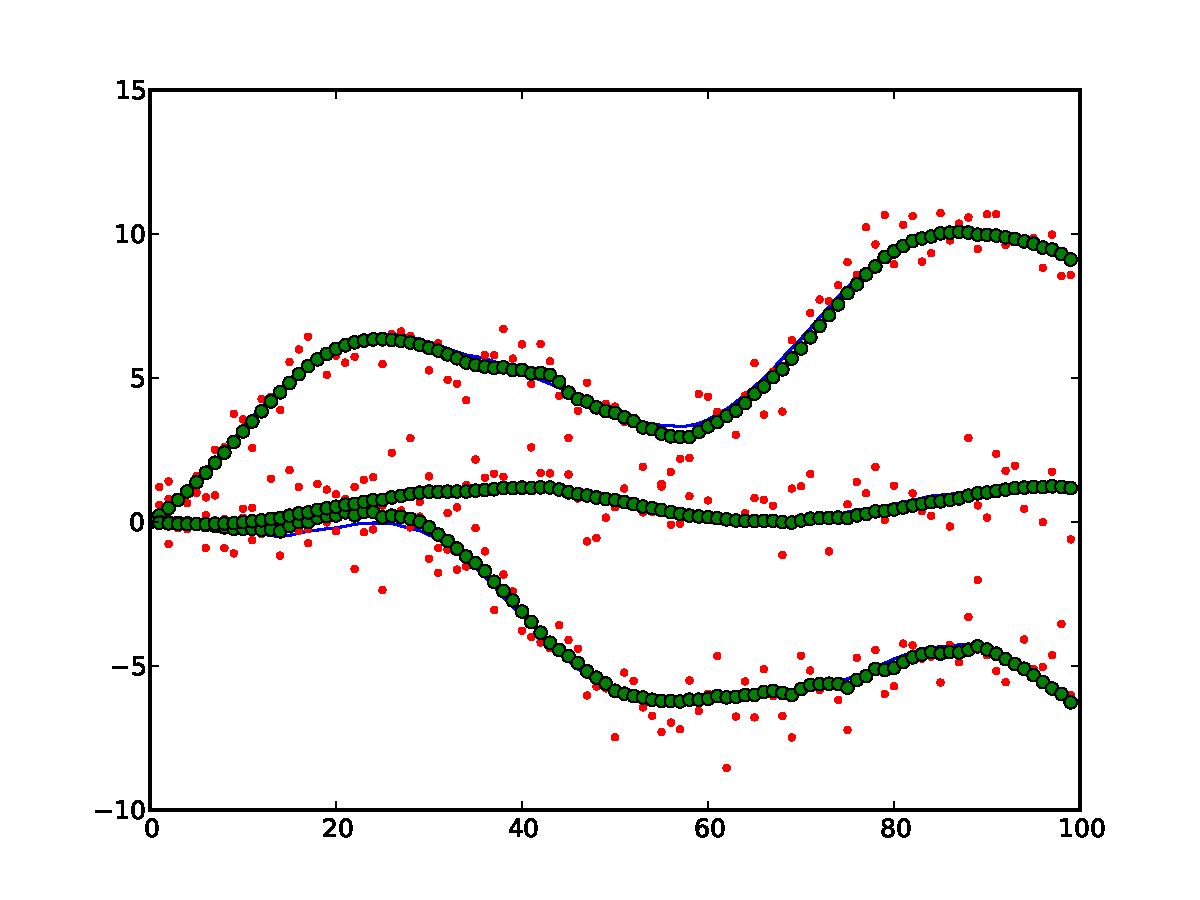
\includegraphics[width=0.6\textwidth,height=\textheight]{AdvFilteringFigures/extendedkalmanfilter1.*}
\caption{The Extended Kalman Filter applied to the motion of a
differential drive robot. Domain axis is time and vertical axis are the
state variables. The simulation pose is given by the blue line, the
observation of the pose given by the red dots and the pose estimate is
given by the green dots.}
\end{figure}

\begin{figure}
\centering
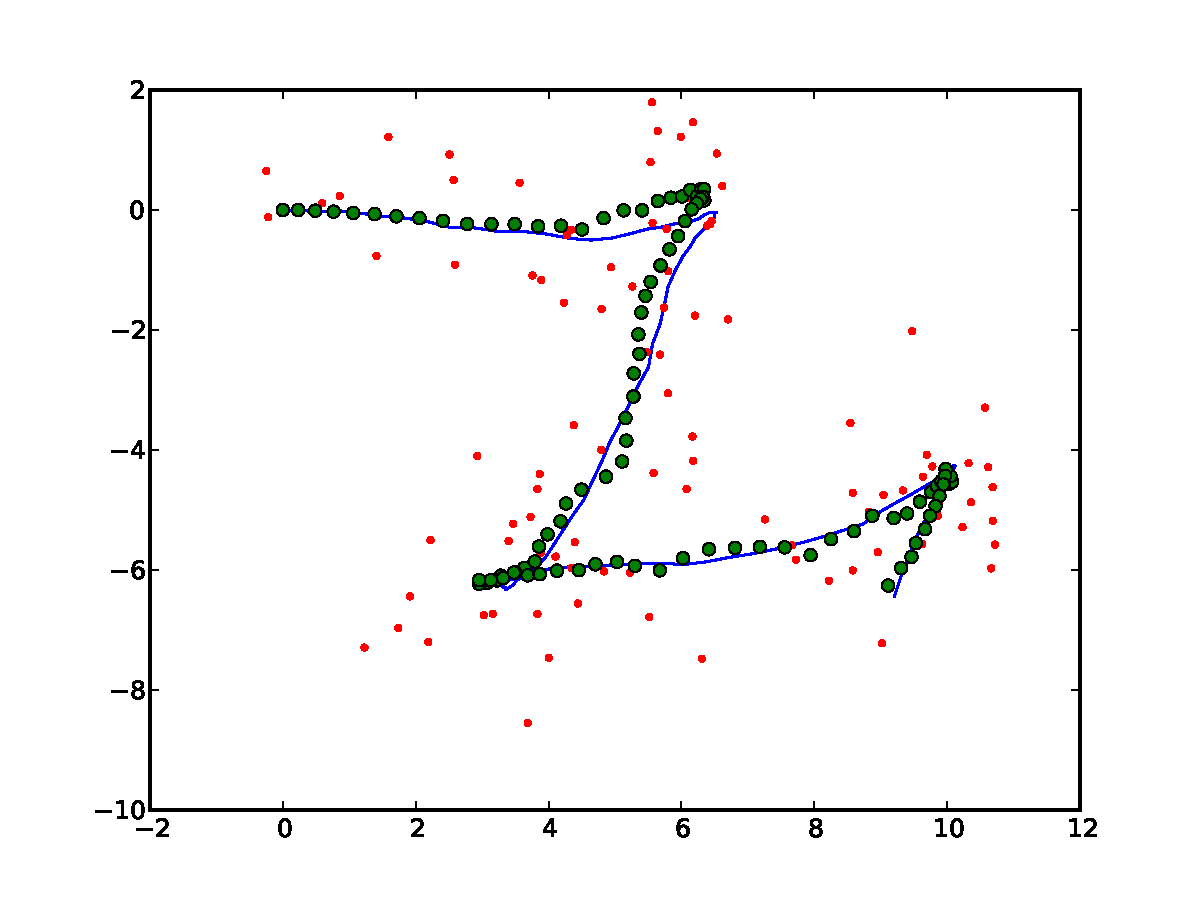
\includegraphics[width=0.6\textwidth,height=\textheight]{AdvFilteringFigures/extendedkalmanfilter2.*}
\caption{The Extended Kalman Filter applied to the motion of a
differential drive robot. This figure plots the \(y\) state variable
against the \(x\) state variable with \(\theta\) ignored. The simulation
pose is given by the blue line, the observation of the pose given by the
red dots and the pose estimate is given by the green dots.}
\end{figure}

\hypertarget{mecanum-ekf-example}{%
\subsection{Mecanum EKF Example}\label{mecanum-ekf-example}}

Developing the Extended Kalman Filter for the Mecanum drive is basically
the same process. The only thing to derive is the matrix \(F\).
Recalling \texttt{meccanumDFK}:

\begin{quote}
\[\begin{aligned}
\begin{bmatrix} x_{k+1}\\[3mm] y_{k+1}\\[3mm] \theta_{k+1} \end{bmatrix}
=   \begin{bmatrix} x_{k}\\[3mm] y_{k}\\[3mm] \theta_{k} \end{bmatrix} +
\frac{ r\Delta t }{4} \begin{bmatrix} A\cos(\theta_{k})  - B \sin(\theta_{k})   \\[3mm]
A\sin(\theta_{k})  + B \cos(\theta_{k})                     \\[3mm]
                            \frac{2}{(L_1+L_2) } C
         \end{bmatrix}
\end{aligned}\]
\end{quote}

where
\(A = \left( \omega_{FL,k} + \omega_{FR,k} + \omega_{BL,k} + \omega_{BR,k} \right)\),
\(B = \left(-\omega_{FL,k} + \omega_{FR,k} + \omega_{BL,k} - \omega_{BR,k}  \right)\),
and
\(C =  \left( -\omega_{FL,k} + \omega_{FR,k} - \omega_{BL,k} +\omega_{BR,k} \right)\).
If we define \(\xi_k = \left( x_{k} , y_{k} , \theta_{k} \right)^T\),
\(u_k =\left(  \omega_{FL,k} , \omega_{FR,k} , \omega_{BL,k} ,\omega_{BR,k} \right)^T\)
and reduce the \(k\) index by one, then the process can be written
compactly as

\[\xi_{k} = f(\xi_{k-1}, u_k) .\]

Computing the Jacobian of \(f\):

\[\begin{aligned}
F = \begin{bmatrix} 1 & 0 & \frac{ r\Delta t }{4}  \left[ - A\sin(\theta_{k-1})  - B\cos(\theta_{k-1})  \right] \\[3mm]
0 & 1 & \frac{ r\Delta t }{4}  \left[ A \cos(\theta_{k-1})  - B \sin(\theta_{k-1})  \right] \\[3mm]
0 & 0 & 1
\end{bmatrix} .
\end{aligned}\]

The rest of the process is identical to the differential drive examples.

\hypertarget{process-noise}{%
\subsection{Process Noise}\label{process-noise}}

We return to our original nonlinear process,

\[x_k = f(u_k,x_{k-1}) + v_k,\]

\[z_k = h(x_{k-1})+w_k\]

where, \(x_k \in R^n\), \(u_k \in R^p\), \(v_k  \in R^n\),
\(w_k  \in R^m\), \(v_k\) has variance \(V_k\) and \(w_k\) has variance
\(W_k\), and let

\[\begin{aligned}
\displaystyle F_k =
  \begin{bmatrix} \frac{\partial f_1}{\partial x_1} & \frac{\partial f_1}{\partial x_2}  & \dots &
\frac{\partial f_1}{\partial x_n}  \\[8pt]
\frac{\partial f_2}{\partial x_1} & \frac{\partial f_2}{\partial x_2}  & \dots &
\frac{\partial f_2}{\partial x_n}  \\[8pt] \vdots & \vdots & \vdots \\[8pt]
\frac{\partial f_n}{\partial x_1} & \frac{\partial f_n}{\partial x_2}  & \dots &
\frac{\partial f_n}{\partial x_n}  \end{bmatrix},
\displaystyle H_k = \begin{bmatrix} \frac{\partial h_1}{\partial x_1} & \frac{\partial h_1}{\partial x_2}  & \dots &
\frac{\partial h_1}{\partial x_n}  \\[8pt]
\frac{\partial h_2}{\partial x_1} & \frac{\partial h_2}{\partial x_2}  & \dots &
\frac{\partial h_2}{\partial x_n}  \\[8pt] \vdots & \vdots & \vdots \\[8pt]
\frac{\partial h_m}{\partial x_1} & \frac{\partial h_m}{\partial x_2}  & \dots &
\frac{\partial h_m}{\partial x_n}  \end{bmatrix}
\end{aligned}\]

How to model the noise? The noise in the controls is the input and it
drives the process noise. We assume here that we are going to gain all
of our noise from the control noise and develop the model. We first
assume that the control noise is drawn from a zero mean normal
distribution with a covariance matrix \(R_k\): \(N(0,R_k)\). We also
assume that the process noise depends on control noise:
\(f(u_k + N(0,R_k) ,x_k)\) . The details are outside the scope of this
text, but we have that a change of coordinates can relate the resulting
process noise \(V_k\) to control noise \(R_k\). The transformation that
relates the noise term \(V_k\) to the covariance \(R_k\) is

\[V_k = G_k R_k G_k^T\]

where \(G_k\) is the Jacobian of \(g_k\) with respect to the control
variables.

\[\begin{aligned}
\displaystyle G_k =
  \begin{bmatrix} \frac{\partial g_1}{\partial u_1} & \frac{\partial g_1}{\partial u_2}  & \dots &
\frac{\partial g_1}{\partial u_p}  \\[8pt]
\frac{\partial g_2}{\partial u_1} & \frac{\partial g_2}{\partial u_2}  & \dots &
\frac{\partial g_2}{\partial u_p}  \\[8pt] \vdots & \vdots & \vdots \\[8pt]
\frac{\partial g_n}{\partial u_1} & \frac{\partial g_n}{\partial u_2}  & \dots &
\frac{\partial g_n}{\partial u_p}  \end{bmatrix}
\end{aligned}\]

\textbf{Example with the DD model:} The linearization of \(g\) with
respect to the control:

\[\begin{aligned}
G =  \frac{\partial g}{\partial u_{k}}=
  \left( \begin{array}{cc}\displaystyle\frac{r\Delta
      t}{2}\cos\theta_k& \displaystyle\frac{r\Delta
    t}{2}\cos\theta_k\\[8pt]\displaystyle\frac{r\Delta
    t}{2}\sin\theta_k& \displaystyle\frac{r\Delta
    t}{2}\sin\theta_k \\[8pt]
  \displaystyle\frac{r\Delta
    t}{2L}& -\displaystyle\frac{r\Delta
    t}{2L} \end{array}\right)
\end{aligned}\]

We can map the control noise into process space via

\[\begin{aligned}
V_k =
\begin{pmatrix}
\displaystyle\frac{r\Delta t}{2}\cos\theta_k& \displaystyle\frac{r\Delta t}{2}\cos\theta_k\\[8pt]
\displaystyle\frac{r\Delta t}{2}\sin\theta_k& \displaystyle\frac{r\Delta  t}{2}\sin\theta_k \\[8pt]
  \displaystyle\frac{r\Delta t}{2L}& -\displaystyle\frac{r\Delta t}{2L}
  \end{pmatrix}
\begin{pmatrix}
\sigma_1^2 & 0 \\[8pt]
0 & \sigma_2^2
\end{pmatrix}
\begin{pmatrix}
\displaystyle\frac{r\Delta t}{2}\cos\theta_k & \displaystyle\frac{r\Delta t}{2}\sin\theta_k & \displaystyle\frac{r\Delta t}{2L} \\[8pt]
\displaystyle \frac{r\Delta t}{2}\cos\theta_k &\displaystyle \frac{r\Delta  t}{2}\sin\theta_k & -\displaystyle\frac{r\Delta t}{2L}
\end{pmatrix}
\end{aligned}\]
